\part{Technical description}
\chapter{Hardware}
\section{Introduction to CSAD}
The CS Arctic Drillship was built and instrumented in 2016, with the intention of facilitating more research on Thruster-Assisted Position Mooring. For an in-depth description of the design and construction process, the reader is referred to \cite{bjorno2016thruster}. 

The vessel is a 1:90 scale model of the Statoil Cat I Arctic Drillship. It is equipped with 6 azimuth thruster (3 fore and 3 aft), in addition to a moon-pool for turret and mooring lines. The main dimensions of the vessel are:
\begin{table}[h!]
	\caption{Main dimensions of CSE1}
	\centering
	\begin{tabular}{cc}
		\hline
		LOA & 2.578[m]\\
		B & 0.440 [m]\\
		D & 0.211[m]\\
		T & 0.133[m]\\
		$\Delta$ & 127.92 [kg]\footnote{The weight displacement is based on design loading condition(design water line)}\\\hline
	\end{tabular}
\end{table}

\subsection{Literature}
The development of CSAD and its systems is a product of research from several theses, which contain complementary information on the theory applied to the system. 
\subsubsection{Journals and conferences}
\begin{itemize}
	\item 
\end{itemize}
\subsubsection{Specialization projects and master theses}
\begin{itemize}
	\item Thruster-Assisted Position Mooring of C/S Inocean Cat I Drillship \citep{bjorno2016thruster}
	\item Constrained Optimal Thrust Allocation for C/S Inocean Cat I Drillship \citep{frederich2016constrained}
	\item Force Field Identification and Positioning Control of an Autonomous Vessel using Inertial Measurement Units \citep{udjus2017}
\end{itemize}

\section{Actuators}
The installed azimuth thrusters are of the type Aero-naut Precision Schottel, with 30 millimeter diameter propellers. They are positioned according to the design of the full-scale ship, as given in Figure \ref{fig:thruster_positions} and Table \ref{tab:thruster_positions}. 
\begin{figure}[htb!]
	\centering
	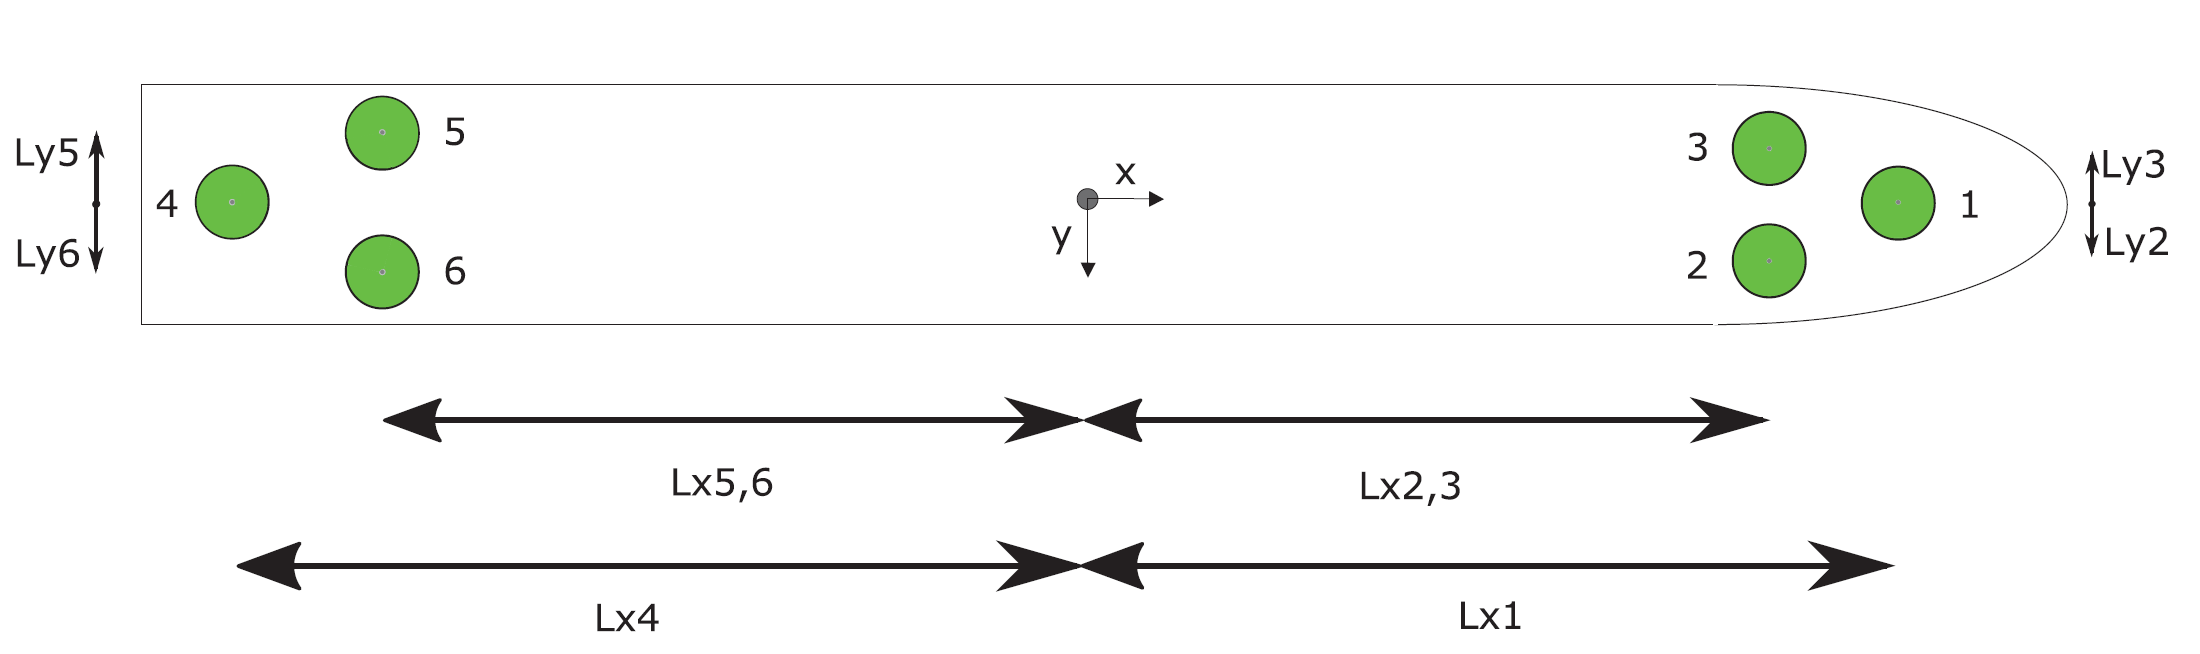
\includegraphics[width=\linewidth]{fig/thruster_position.png}
	\caption{Illustration of thruster positions. Adapted from \cite{frederich2016constrained}}
	\label{fig:thruster_positions}
\end{figure}
\begin{table}[htb!]
	\centering
	\caption{Thruster positions}
	\label{tab:thruster_positions}
	\begin{tabular}{ccc}
		\hline
		\textbf{Thruster} & \textbf{Position X}[m] & \textbf{Position Y}[m]\\ \hline
		Thruster 1 & 1.0678 & 0.0\\
		Thruster 2 & 0.9344 & 0.11\\
		Thruster 3 & 0.9344 & -0.11\\
		Thruster 4 & -1.1644 & 0.0\\
		Thruster 5 & -0.9911 & -0.1644\\
		Thruster 6 & -0.9911 & 0.1644\\ \hline
	\end{tabular}
\end{table}

In \cite{frederich2016constrained}, the thrust coefficients were estimated based on bollard pull tests. The values given in Table \ref{tab:thruster_coefficients} are mean values from the tests, due to discrepancies in the bollard pull test at low thrust commands. 
\begin{table}[htb!]
	\centering
	\caption{Thruster coefficients}
	\label{tab:thruster_coefficients}
	\begin{tabular}{ccccccc}
		\hline
		 & \textbf{Thruster 1} & \textbf{Thruster 2} & \textbf{Thruster 3} & \textbf{Thruster 4} & \textbf{Thruster 5} & \textbf{Thruster 6}\\ \hline
		$K_T$ & 0.3763 & 0.3901 & 0.3776 & 0.5641 & 0.4799 & 0.5588\\
		$K_Q$ & 0.0113 & 0.0117 & 0.0113 & 0.0169 & 0.0144 & 0.0168\\ \hline
	\end{tabular}
\end{table}

\section{Power system}
The vessel is powered through six 12V 12Ah batteries, connected in parallel. Figure \ref{fig:power_system} show a schematic drawing of the power system.

\begin{figure}[h!]
	\centering
	\begin{subfigure}{0.3\textwidth}
		\centering
		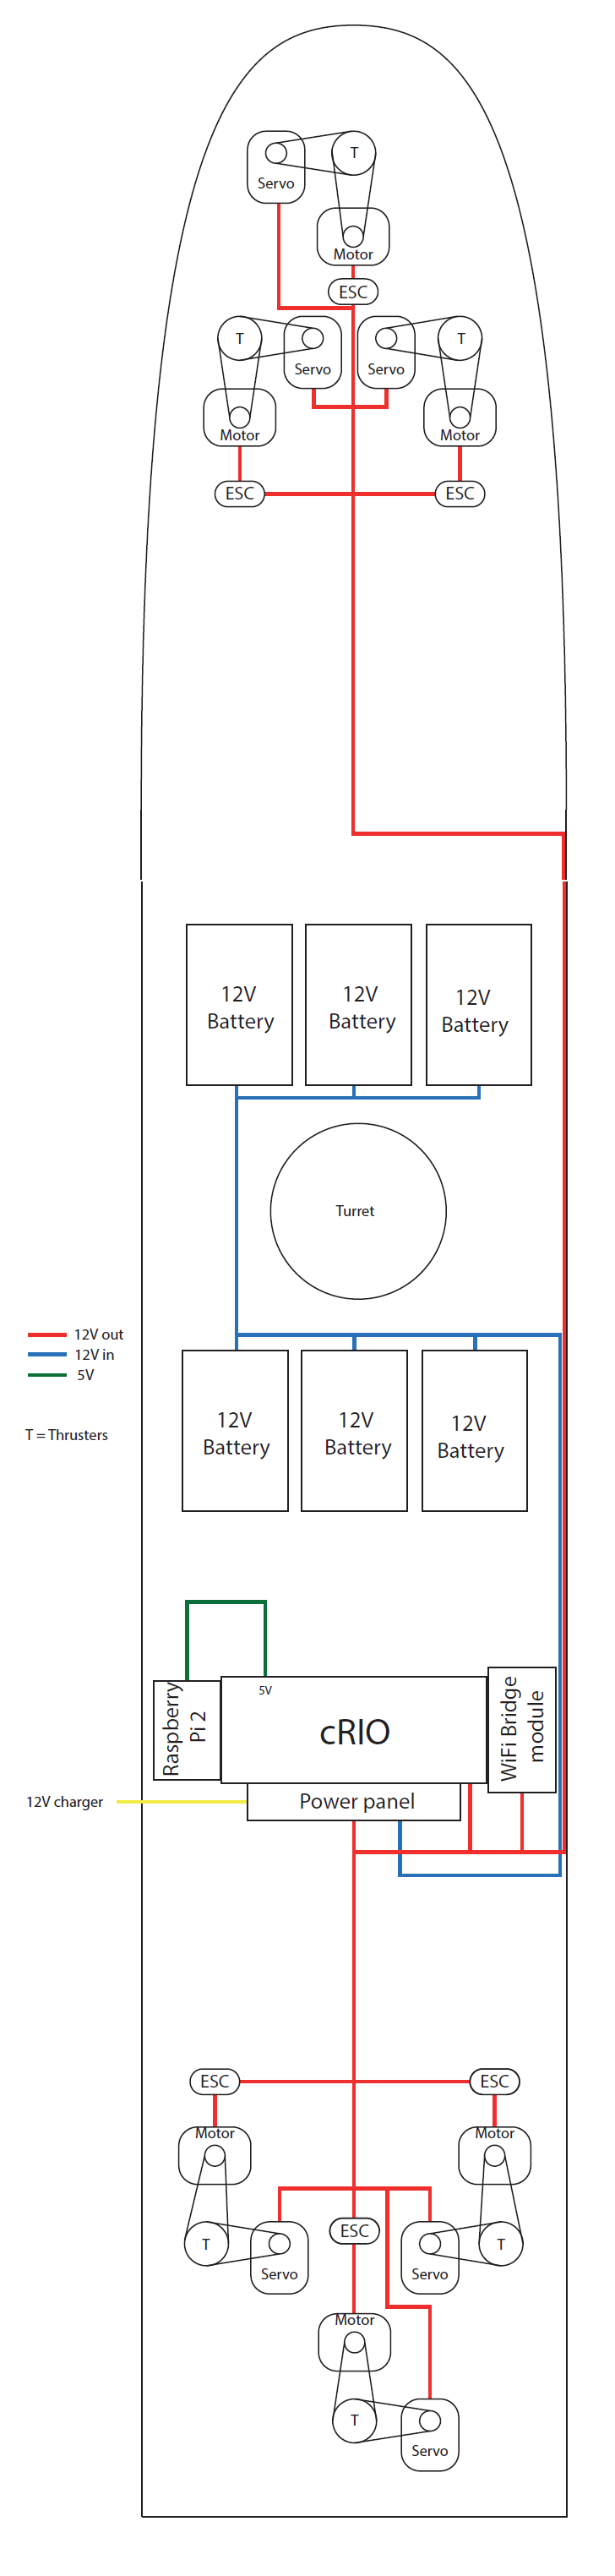
\includegraphics[height=0.9\textheight]{fig/power_system.png}
		\caption{Power system}
		\label{fig:power_system}
	\end{subfigure}
\qquad \qquad
	\begin{subfigure}{0.3\textwidth}
		\centering
		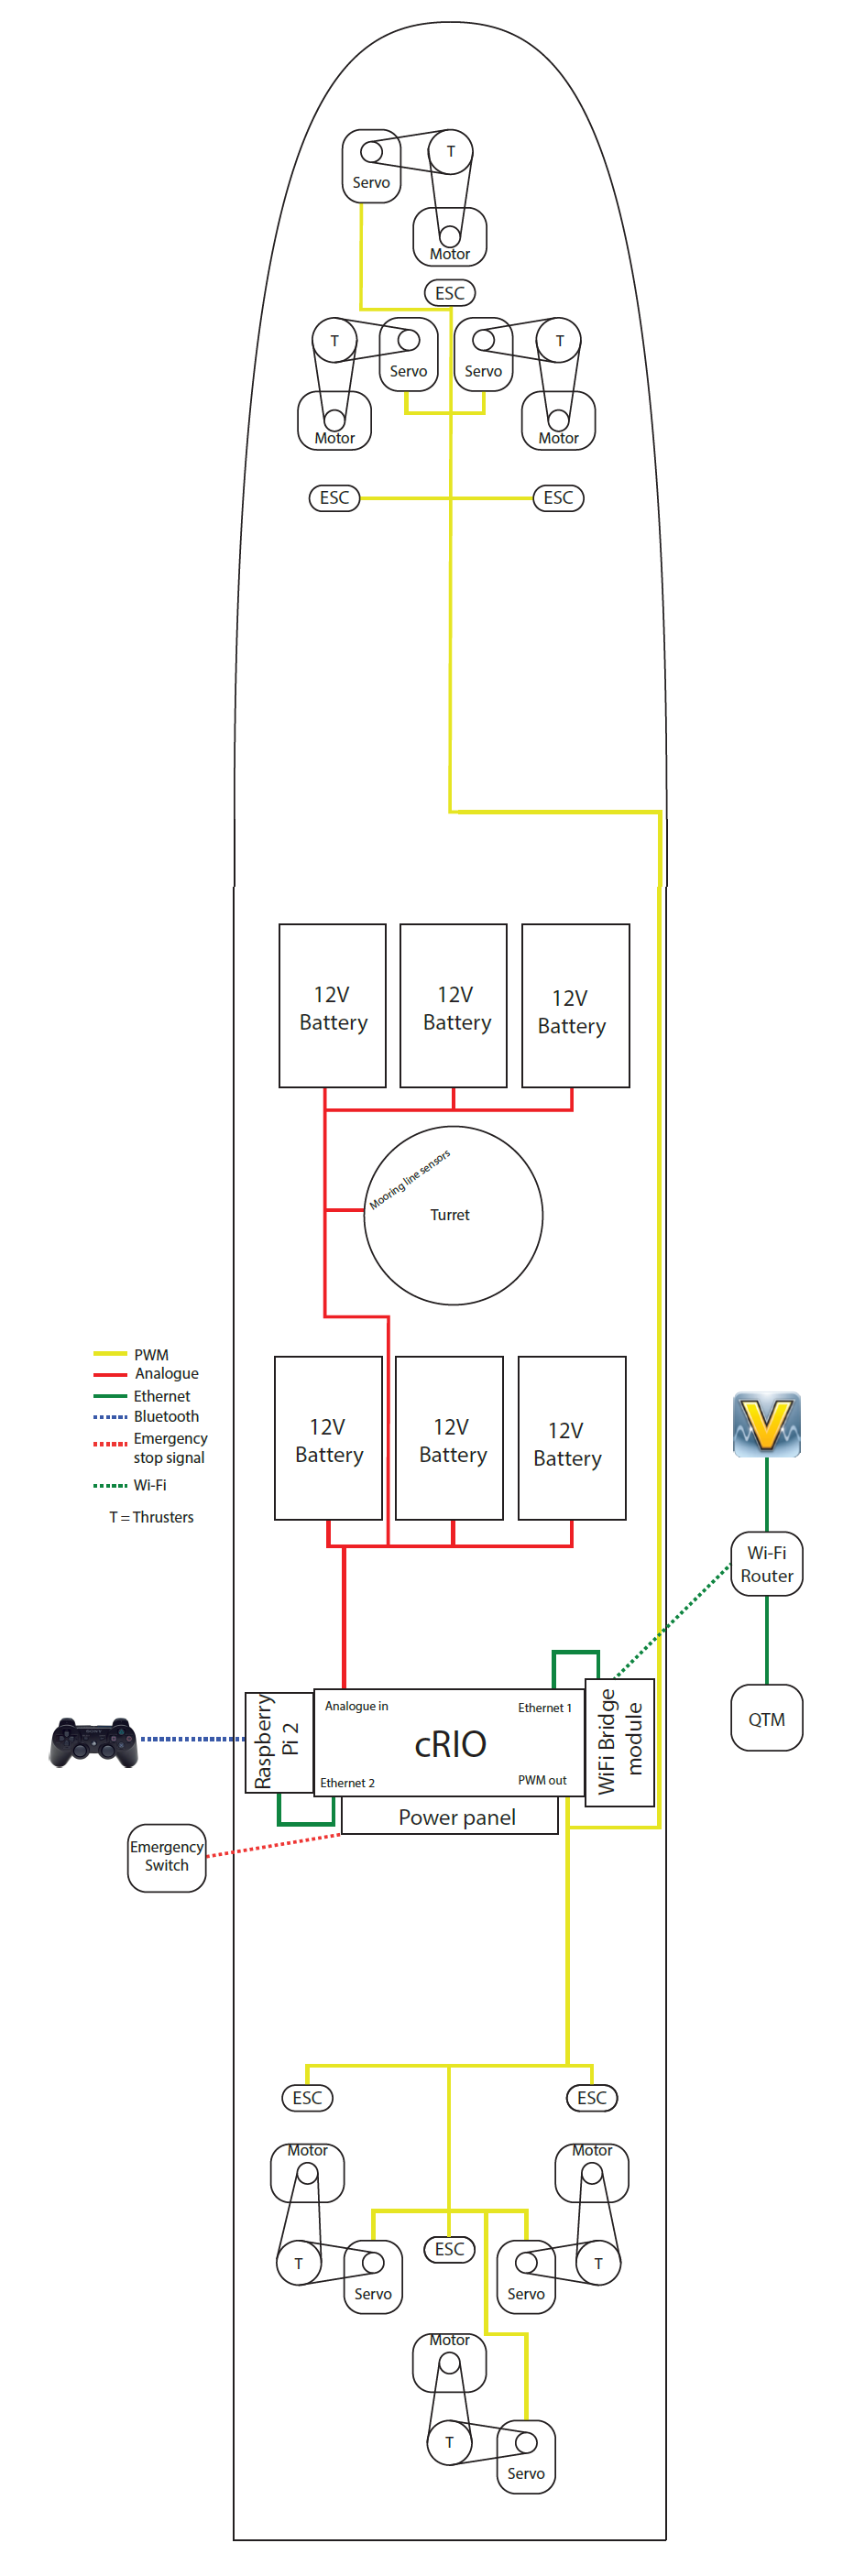
\includegraphics[height=0.9\textheight]{fig/control_system.png}
		\caption{Control system}
		\label{fig:control_system}
	\end{subfigure}
\caption{Illustration of power and control system. Figures adapted from \cite{bjorno2016thruster}.}
\label{fig:power_and_control_system}
\end{figure}
\section{IMU}
CSAD is equipped with one Inertial Measurement Unit (IMU) from Analog Devices. The sensor mounted on-board is the ADIS16364 and includes a triaxis gyroscope and triaxis accelerometer. The sensor has built-in compensation for bias, alignment and sensitivity, and provides accurate measurements over a temperature range of -10 to +70 degrees Celsius. The most relevant data is presented in Table \ref{tab:IMU_specifications}, and for supplementary information the reader is referred to the data sheet \cite{adis16364}. The reference frame of the sensor is illustrated in Figure \ref{fig:IMU_reference_frame}, with positive directions illustrated by arrows. As seen, the standard reference frame for linear accelerations uses left-hand orientation, while the angular rates uses right-hand orientation. It is advised to change the reference frame of accelerations to right-hand, which is achieved by multiplying the accelerations with -1. Note that this also changes the positive direction, defined as the direction of acceleration that produces a positive output. 
\begin{table}[htb!]\caption{IMU specifications}\label{tab:IMU_specifications}
	\centering
	\begin{tabular}{c|c|c|c|}
		\cline{2-4}
		& \textbf{Parameter} & \textbf{Typical value} & \textbf{Unit}\\ \cline{1-4}
		\multicolumn{1}{|c|}{\multirow{5}{*}{\textbf{Gyroscopes}}} & Dynamic range & $\pm 350$ & $^{o}$/sec\\ 
		\multicolumn{1}{|c|}{} & Sensitivity & 0.0125 & $^{o}$/sec/LSB\\ 
		\multicolumn{1}{|c|}{} & Bias stability, $\sigma$ & 0.007 & $^{o}$/sec\\ 
		\multicolumn{1}{|c|}{} & Angular random walk & 2.0 & $^{o}$/$\sqrt{hr}$\\ 
		\multicolumn{1}{|c|}{} & Output noise & 0.8 & $^{o}$/sec rms\\ \cline{1-4}
		
		\multicolumn{1}{|c|}{\multirow{5}{*}{\textbf{Accelerometers}}} & Dynamic range & $\pm 5.25$ & g\\ 
		\multicolumn{1}{|c|}{} & Sensitivity & 1.00 & mg/LSB\\ 
		\multicolumn{1}{|c|}{} & Bias stability, $\sigma$ & 0.1 & mg\\ 
		\multicolumn{1}{|c|}{} & Velocity random walk & 0.12 & m/sec/$\sqrt{hr}$\\ 
		\multicolumn{1}{|c|}{} & Output noise & 5 & mg rms\\ \cline{1-4}
		
		\multicolumn{1}{|c|}{\multirow{1}{*}{\textbf{Power supply}}} & Operating voltage& $5.0 \pm 0.25$ & V\\ \cline{1-4}
	\end{tabular}
\end{table}
\begin{figure}[htb!]
	\centering
	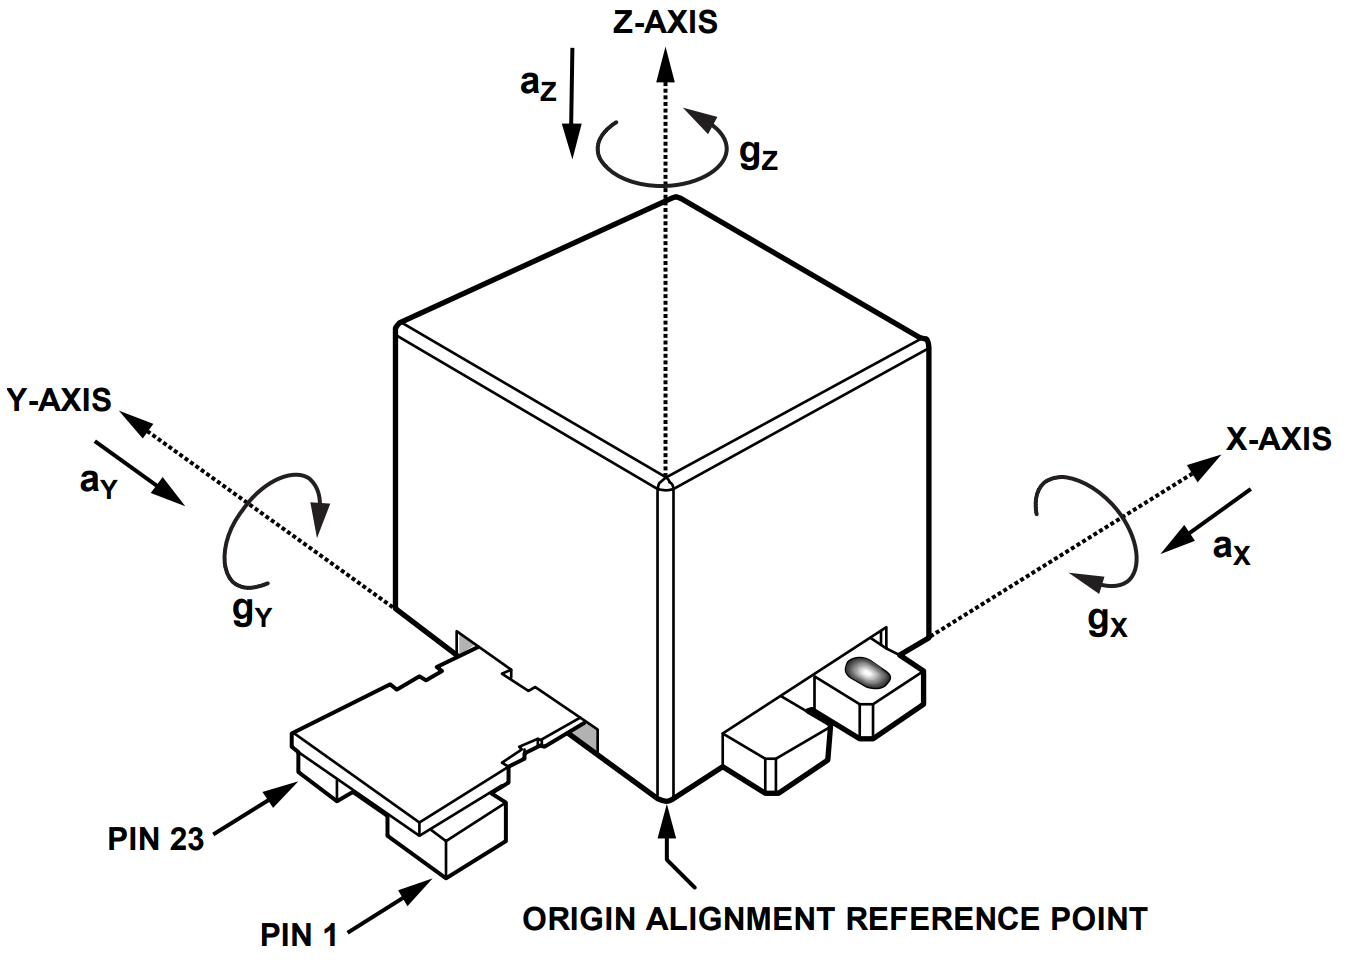
\includegraphics[width=0.6\linewidth]{fig/IMU_reference_frame.png}
	\caption{IMU reference frame from manufacturer}
	\label{fig:IMU_reference_frame}
\end{figure}

\section{Control system}
The on-board control system is illustrated in Figure \ref{fig:control_system}, and consists of the following parts:
\begin{itemize}
	\item one National Instruments compact reconfigurable input/output (cRIO) embedded controller
	\item one Raspberry Pi (RPi) single-board computer
	\item six electronic speed controllers (ESC) connected to six motors controlling thruster speed
	\item six servos controlling thruster angle
\end{itemize}
For complementary information on the ESC, motors, servos and PWM signals, see \cite{bjorno2016thruster}.
\subsection{cRIO}
The model on-board is the cRIO-9024, and it is connected to 4 FPGA modules for analog and digital I/O:
\begin{itemize}
	\item One NI-9215, Analog input
	\item Two NI-0237, Analog bridge
	\item Two NI-9401, Bidirectional digital input
	\item One NI-9411, Digital input
	\item One NI-9474, Digital output
	\item One NI-9871, Serial interface
\end{itemize}
\subsection{RPi}
The Raspberry Pi provides communication with the Siaxaxis controller, as described in Section \ref{sec:high_level_communication}. It works as an embedded system, and once powered it will start connecting to the wireless controller. When connection is established, it continuously sends the Sixaxis controller output to the cRIO over Ethernet. 

If there are problems establishing connection between Sixaxis and RPi, try restarting the RPi. If this doesn't work, contact Torgeir Wahl or see the MCLab Handbook on Github for description on how to reconfigure the RPi.
\subsection{ESC and DC-motor}
The ESC's are of the type O.S. OCA-150 50 A BL, connected to brushless UMA-2820-950 DC motors driving the thrusters. The ESC's are controlled with PWM signals. As the motors are much more powerful than desired for the model, the PWM signal is constrained. Table \ref{tab:PWM_constraints} gives the constraints on the PWM signal. \todo{Verify the PWM constraints}
\begin{table}[htb!]
	\centering
	\caption{PWM constraints}
	\begin{tabular}{ccc}
		\hline
		\textbf{Direction} & \textbf{Signal range PWM} & Tick\\ \hline
		Full reverse & 6.25 [\%] & 50.000\\
		Neutral & 7.5 [\%] & 60.000\\
		Full forward & 8.75 [\%] & 70.000\\ \hline
	\end{tabular}
	\label{tab:PWM_constraints}
\end{table}
\subsection{Servo}
The servos controlling the thruster angles are of the type Dynamixel MX-106R, and are geared 1:1 with the thrusters(1 degree turn on servo results in 1 degree on thruster). The servos are manually tuned to have a zero-angle offset in initial start. As of July 2017, the initial offsets are given in Table \ref{tab:angle_offset}. Maximum and minimum angles for all servos are given in \eqref{eq:maxmin_angle}. If one thruster reaches maximum/minimum angle, it is reset to initial neutral position, as described in the software section. For complementary information.  \todo{update min/max values on PWM in init file}
\begin{equation}\label{eq:maxmin_angle}
	\bm{\alpha} \in [-10240\degree, 10240\degree]
\end{equation}
\begin{table}[htb!]
	\centering
	\caption{Servo angle offset}
	\begin{tabular}{cc}
		\hline
		\textbf{Thruster} & \textbf{Offset}\\ \hline
		$\alpha_1$ & -149\degree\\
		$\alpha_2$ & 50\degree\\
		$\alpha_3$ & 5\degree\\
		$\alpha_4$ & -17\degree\\
		$\alpha_5$ & 127\degree\\
		$\alpha_6$ & -36\degree\\
		\hline
	\end{tabular}
\label{tab:angle_offset}
\end{table}

\section{High-level communication}\label{sec:high_level_communication}
\begin{figure}[htb!]
	\centering
	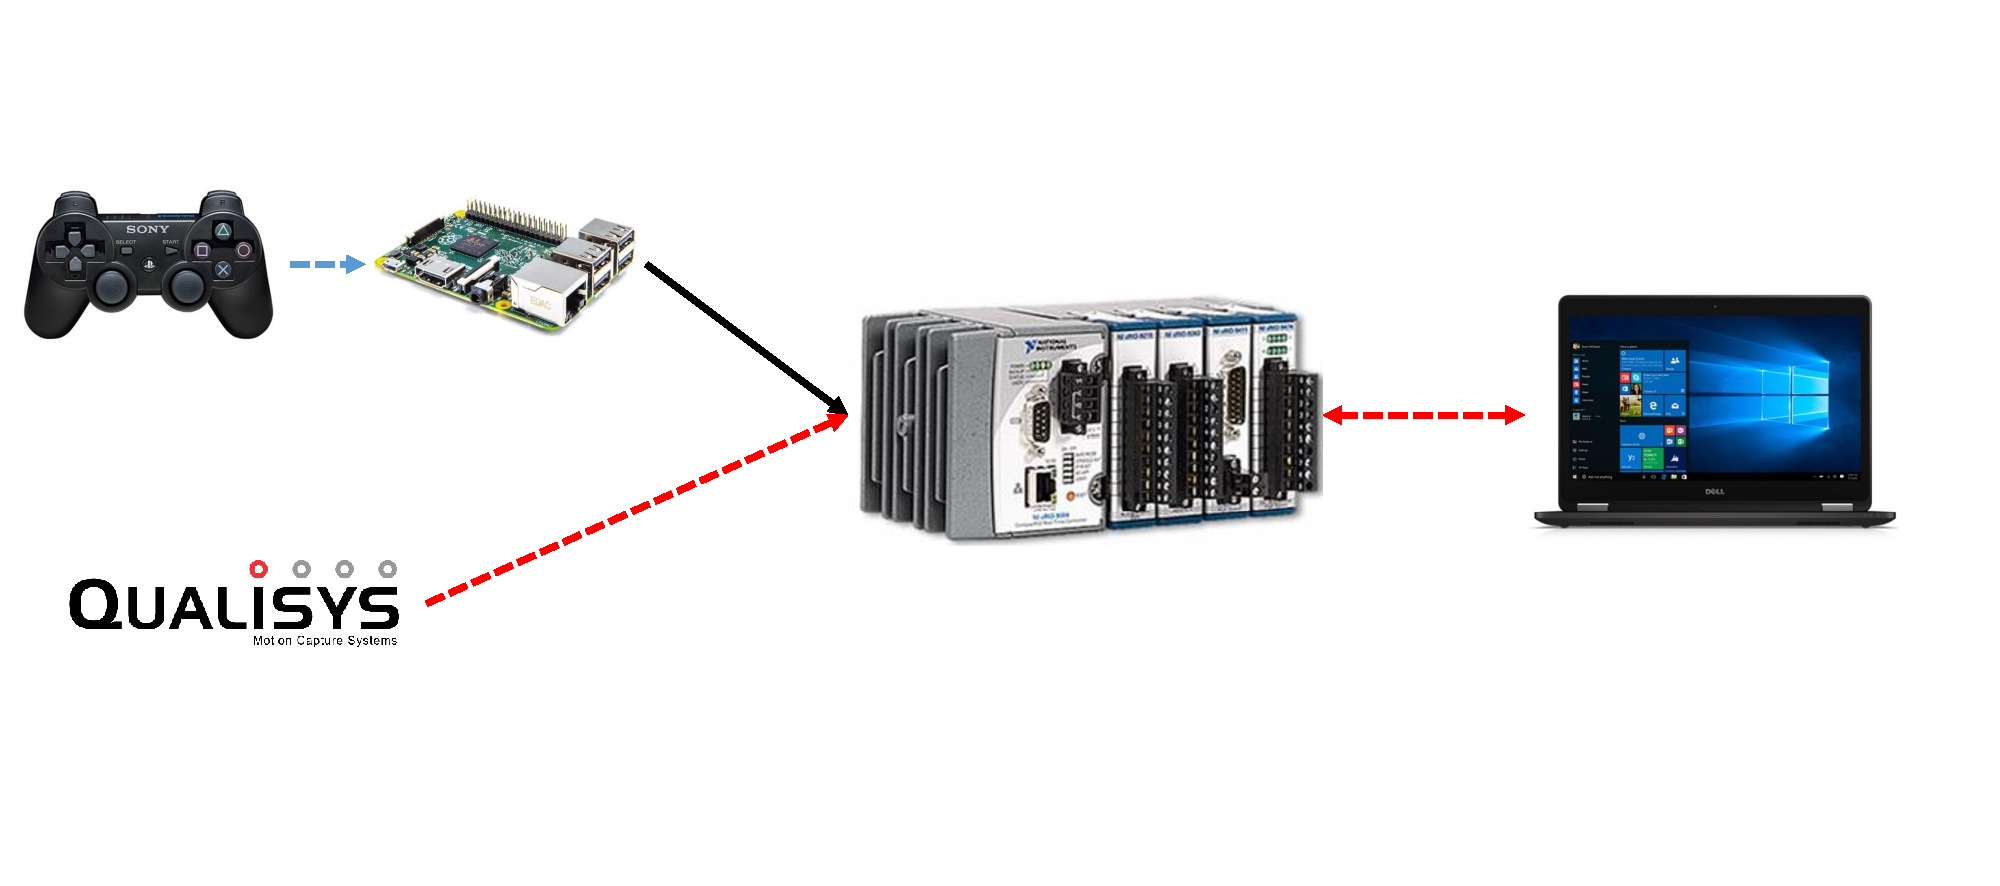
\includegraphics[width=\textwidth]{fig/high-level_control.pdf}
	\caption{CSE1 communication diagram}
	\label{fig: CSE1 communication}
\end{figure}
Following Figure \ref{fig: CSE1 communication} from left to right:
\begin{description}
	\item [{Sixaxis}] transmits its Joystick information to the RPi over Bluetooth communication. 
	\item [{RPi}] receives Sixaxis data through the USB dongle and forwards it using Ethernet connection (TCP).
	\item [{cRIO}] reads QTM broadcast positioning data through the Wi-Fi bridge on Ethernet port 1, Sixaxis data on Ethernet port 2. Online data and laptop input is transmitted and received on Ethernet port 1 by the VeriStand Engine.
	\item [{Laptop}] reads simulation data and sends input to the cRIO over MC Lab Wi-Fi.
\end{description}
Hence, there are two possible methods for controlling the vessel:
\begin{itemize}
	\item laptop connected to the MC Lab wireless network
	\item Sixaxis wireless gamepad(labeled \textit{CSAD})
\end{itemize}


\chapter{Software}
\section{Introduction}
In order to control CSAD, there are several software parts that runs. This chapter gives a description of the software topology on CSAD. Note that the software is ready to use, and alterations in the software described here is not necessary(except modifying \textit{ctrl\textunderscore custom}, see Part \ref{part2}).
\section{Control system}
Figure \ref{fig: CSE1 software} illustrate the software architecture, and gives an overview on how the different modules and I/O from the Simulink models are connected in VeriStand. In general, the software can be divided into 2 groups: 
\begin{itemize}
	\item[MATLAB] generated parts: ctrl\textunderscore custom, ctrl\textunderscore TAPM, ctrl\textunderscore sixaxis2thruster, STOP and u2pwm
	\item[LabVIEW] generated parts: IMU, Oqus, WL\textunderscore Joystick and FPGA
\end{itemize}
All of these modules are described in the latter. 
\begin{figure}[htb!]
	\centering
	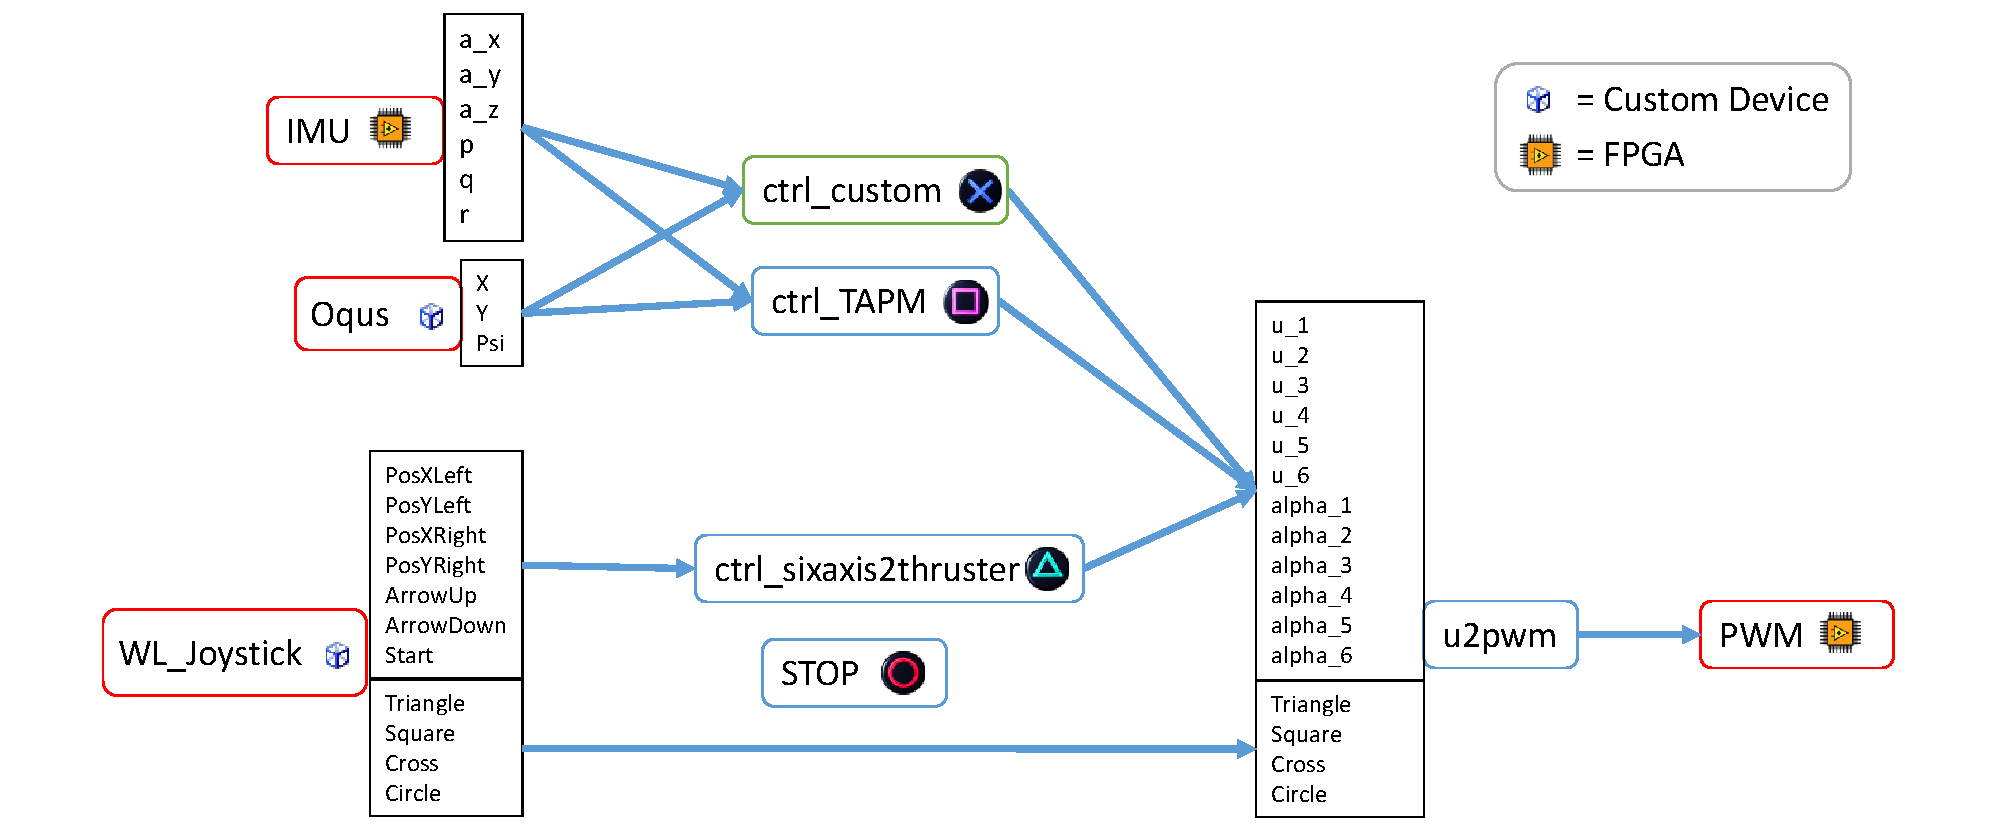
\includegraphics[width=\textwidth]{fig/software_overview.pdf}
	\caption{CSE1 control software}
	\label{fig: CSE1 software}
\end{figure}

\subsection{ctrl\textunderscore custom}
This is the only reconfigurable software, and does not consist of any control system. In Part \ref{part2} a description on how to configure and upload the code to CSAD is given. 
\subsection{ctrl\textunderscore TAPM}
This code is a basic TAPM control system, intended for demonstrations of the vessel. The desired position of the vessel is modified in VeriStand. 
\subsection{ctrl\textunderscore sixaxis2thruster}
All 6 thruster can be controlled manually using the Sixaxis controller. The right joystick controls the direction of the three thrusters aft, while the left joystick controls the front thrusters. ArrowUp and ArrowDown sets the thrust limits, and  Start resets the limitation to 0. 

\subsection{STOP}
This system simply stops the vessel, by setting the thrust of all thrusters to 0. 
\subsection{u2pwm}
This code transforms the control input to PWM signals, which are sent to the FPGA module. There are 2 groups of inputs, namely the control signal and a switch signal. The switch signal is used to switch between the 4 control systems described previously. Switching is simply achieved by pressing either one of the four symbols, and the mapping between the buttons and models is shown in Figure \ref{fig: CSE1 software}. The code is not supposed to be altered, and should work as it is. 

\subsubsection{Switch}
The switch simply forward the input from the desired model, as given by the switch signal:
\begin{itemize}
	\item ctrl\_sixaxis2thruster when 
\includegraphics[scale=0.4]{fig/sixaxis_triangle} is pushed
	\item ctrl\_sixaxis2direction when 
\includegraphics[scale=0.4]{fig/sixaxis_square} is pushed
	\item ctrl\_DP when 
\includegraphics[scale=0.4]{fig/sixaxis_circle} is pushed
	\item ctrl\_student when 
\includegraphics[scale=0.4]{fig/sixaxis_cross} is pushed
\end{itemize}
\subsubsection{Saturation}

\subsubsection{Low-pass}
\subsubsection{Mapping}

\subsection{Oqus}
The Qualisys Track Manager software broadcast the position data of the vessel over MC Lab Wifi. Reading these data is done on the cRIO through a Custom Device module named Oqus. The Oqus software simply listen to the network for data from QTM, and once it receives data it forward the position and orientation to the models as given in Figure \ref{fig: CSE1 software}. The Custom Device is programmed by Torgeir Wahl, and can be found on GitHub. 
\subsection{WL\textunderscore Joystick}
This is the second Custom Device that runs on the cRIO, which listen to the Ethernet 2 port for input from the RPi. It forwards this data to the respective models as given in Figure \ref{fig: CSE1 software}. The software is designed by Torgeir Wahl, and can be found on GitHub. 
\subsection{FPGA}
For the CSE1, 3 FPGA modules are in use(1 for analog signals, 1 for digital signals and 1 for reading IMU data). The FPGA software is described in the MC Lab Software Handbook, and provides a guide on how to create an FPGA module. The modules can be found on GitHub, but are as standard. The PWM signal is mapped as described in Table

\section{Connecting software}
All the different software parts described in the previous Section are connected together in VeriStand. On CSAD, VeriStand 2017 is used. In the system definition file \textit{CSE1.nivssddf}, all necessary mappings of variables are done. In addition, here the different Custom Devices, FPGA code and Simulink Models can be included. However, the standard setup should not be altered, as all necessary code and mappings is already taken care of. For description on how to implement the modified ctrl\textunderscore student Simulink model, the reader is referred to Part \ref{part2}. 
\chapter{Modeling}
The mathematical model of CSE1 is given here, based on system identification done in previous Master's Theses. The model is valid for low-speed. The proposed control design model is
